\section{Methodology}
The general approach taken to prune an optimally trained neural network in the present work is to create a ranked list of all the neurons in the network based off of one of the 3 proposed ranking criteria: Brute Force approximation (which we use as our ground truth), linear approximation and quadratic approximation of the neuron's impact on the overall performance of the network. We then test the effects of removing neurons sequentially on the accuracy of the network. These tests can be found in the Experiments section. Next, we propose our algorithm with 2 variants

\subsection{Brute Force Removal Approach}
This is perhaps the most naive yet the most accurate method for pruning the network. It is also the slowest and hence unusable on large-scale neural networks with thousands of neurons. The idea is to manually check the effect of every single neuron on the output. This is done by running a forward propagation on the validation set $K$ times (where $K$ is the total number of neurons in the network), turning off exactly one neuron each time (keeping all other neurons active) and noting down the change in error. Turning a neuron off can be achieved by simply setting its output to 0. This results in all the outgoing weights from that neuron being turned off. This change in error is then used to generate the ranked list. 

\subsubsection{Taylor Series Representation of Error}
Let us denote the total error from the optimally trained neural network for any given validation dataset with $N$ instances as $\Etotal$. Then,
\begin{align}
\Etotal = \sum_n E_n,
\end{align}
where $E_n$ is the error from the network over one validation instance. $E_n$ can be seen as a function $O$, where $O$ is the output of any general neuron in the network (In reality this error depends on each neuron's output, but for the sake of simplicity we use $O$ to represent that). This error can be approximated at a particular neuron's output (say $O_k$) by using the 2nd order Taylor Series as,

\begin{align}
\hat E_n(O) \approx E_n(O_k) + (O-O_k)\cdot \left.\pdv{E_n}{O}\right|_{O_k} +  0.5\cdot (O-O_k)^2\cdot \left.\pdv[2]{E_n}{O}\right|_{O_k}\label{eq:ts1},
\end{align}

where $\hat E_n(O_k)$ represents the contribution of a neuron $k$ to the total error $E_n$ of the network for any given validation instance $n$. When this neuron is pruned, its output $O_k$ becomes 0. From equation \ref{eq:ts1}, the contribution $E_n(0)$ of this neuron, then becomes:

\begin{align}
\hat E_n(0) \approx E_n(O_k) - O_k\cdot \left.\pdv{E_n}{O}\right|_{O_k} +  0.5\cdot O_k^2\cdot \left.\pdv[2]{E_n}{O}\right|_{O_k}\label{eq:ts2}
\end{align}

Replacing $O$ by $O_k$ in equation \ref{eq:ts1} shows us that the error is approximated perfectly by equation \ref{eq:ts1} at $O_k$. Using this and equation \ref{eq:ts2} we get:

\begin{align}
\Delta E_{n,k} = \hat E_n(0) - \hat E_n(O_k)= - O_k\cdot \left.\pdv{E_n}{O}\right|_{O_k} + 0.5\cdot O_k^2\cdot \left.\pdv[2]{E_n}{O}\right|_{O_k}\label{eq:ts3},
\end{align}

where $\Delta E_{n,k}$ is the change in the total error of the network given a validation instance $n$, when exactly one neuron ($k$) is turned off.


\subsection{Linear Approximation Approach}
\begin{figure}[bh!]
\centering
\newcommand{\repSigmoid}{$\sigma(\cdot)$}
\newcommand{\repLinear}{$\sum$}
\newcommand{\repMse}{MSE}
\newcommand{\repFirstSum}{$\Input j 1$}
\newcommand{\repLastSum}{$\Input i 0$}
\newcommand{\repFirstOutput}{\hspace{1.5cm}$\Con j i 0 \!=\! \Weight j i 0 \Out j 1$}
\newcommand{\repLastOutput}{$\Out i 0$}
\newcommand{\repLoss}{$E$}
\def\svgwidth{0.9\textwidth}
\hspace{-2cm}
\import{}{drawing.pdf_tex}
\hspace{-2cm}
\caption{A computational graph of a simple feed-forward network illustrating the naming of different variables, where $\sigma(\cdot)$ is the nonlinearity, MSE is the mean-squared error cost function and $E$ is the overall loss.}
\label{fig:comp_graph}
\end{figure}
We define the following network terminology here which will be used in this section and all subsequent sections  unless stated otherwise. Figure \ref{fig:comp_graph} can be used as a reference to the terminology defined here:

\begin{align}
E &= \frac{1}{2}\sum\limits_i (\Out i 0 - \Target i)^2 &
\Out i m &= \sigma(\Input i m) &
\Input i m &= \sum\limits_j {\Weight j i m}{ \Out j {m + 1}} &
\Con j i m = \Weight j i m \Out j {m+1}\label{eq:term}
\end{align}
Superscripts represent the index of the layer of the network in question, with 0 representing the output layer. $E$ is the squared-error network cost function. $\Out i m$ is the $i$th output in layer $m$ generated by the activation function $\sigma$, which in this paper is is the standard logistic sigmoid. $\Input i m$ is the weighted sum of inputs to the $i$th neuron in the $m$th layer, and $\Con j i m$ is the contribution of the $j$th neuron in the $(m+1)$th layer to the input of the $i$th neuron in the $m$th layer. $\Weight j i m$ is the weight between the $j$th neuron in the $(m+1)$th layer and the $i$th neuron in the $m$th layer.

We can use equation \ref{eq:ts3} to get the linear error approximation of the change in error due to the $k$th neuron being turned off and represent it as $\Delta E_{k}^1$ as follows:

\begin{align}
\Delta E_{k}^1 = - o_k\cdot \left.\pdv{E}{{\Out j {m+1}}}\right|_{o_k}
\end{align}

The derivative term above is the first-order gradient which represents the change in error with respect to the output of a given neuron $o_j$ in the $(m+1)$th layer. This term can be collected during back-propagation. The derivative term above can be calculated as follows:

\begin{align}
\pdv{E}{{\Out j {m+1}}} = \sum\limits_i \pdv{E}{\Input i m}\cdot \Weight j i m
\end{align}

The full step-by-step mathematical derivation of the above equation can be found in the appendix.
\subsection{Quadratic Approximation Approach}

As seen in equation \ref{eq:ts3}, $\Delta E_{n,k}$ which can now be represented as $\Delta E_{k}^2$ is the quadratic approximation of the change in error due to the $k$th neuron being turned off. The quadratic term in equation \ref{eq:ts3} requires some discussion which we provide here. A more detailed and step-by-step mathematical derivation can be found in the appendix.

Let us reproduce equation \ref{eq:ts3} in our new terminology here: 
\begin{align}
\Delta E_{k}^2 = - o_k\cdot \left.\pdv{E}{{\Out j {m+1}}}\right|_{o_k} + 0.5\cdot o_k^2\cdot \left.\pdv[2]{E}{{\Out j {m+1}}}\right|_{o_k}\
\end{align}

The second term here involves the second-order gradient which represents the second-order change in error with respect to the output of a given neuron $o_j$ in the $(m+1)$th layer. This term can be generated by performing back-propagation using second derivatives. A full derivation of the second derivative back-propagation can be found in the appendix. We will quote some results from the derivation here. The second-order derivative term can be represented as:

\begin{align}
\pdv[2]{E}{{\Out j {m+1}}} &= \sum_i
\pdv[2]{E}{{\Con j i m}} \left({\Weight j i m}\right)^2
\end{align} 

Here,$\Con j i m$ is one of the component terms of $\Input i m$, as follows from the equations in \ref{eq:term}. Hence, it can be easily proved that (full proof in appendix):
\begin{align}
\pdv[2]{E}{{\Con j i m}} = \pdv[2]{E}{{\Input i m}}
\end{align}

Now, the value of $\Input i m$ can be easily calculated through the steps of the second-order back-propagation using Chain Rule. The full derivation can again, be found in the appendix.
\begin{align}
\pdv[2]{E}{{\Input i m}}=\pdv[2]{E}{{\Out i m}} \left(\sigma^{\prime}\left({\Input i m}\right)\right)^2
+
\pdv{E}{{\Out i m}}\sigma^{\prime\prime}\left(\Input i m\right)
\end{align}

\subsection{Proposed Pruning Algorithm}
\begin{figure}
  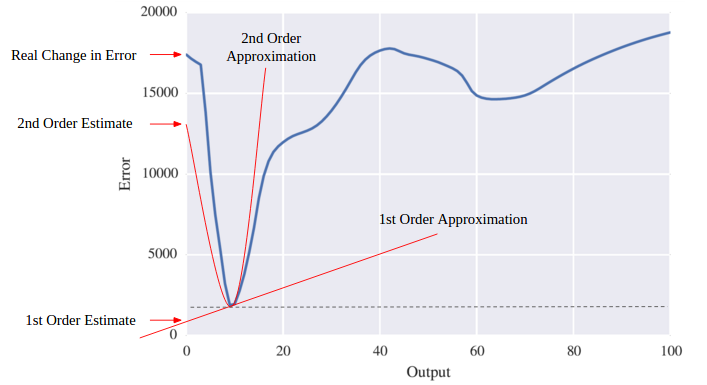
\includegraphics[width=\linewidth]{png/intuition.png}
  \caption{The intuition behind neuron pruning decision.}
  \label{fig:intuition}
\end{figure}

Figure \ref{fig:intuition} shows a random error function plotted against the output of any given neuron. Note that this figure is for illustration purposes only. The error function is minimized at a particular value of the output as can be seen in the figure. This output is fixed during training as decided by back propagation. Pruning this particular neuron would result in a change in the total error that would be equal to the increase shown in the figure. This neuron is clearly a bad candidate for removal. The straight red line in the figure represents the first-order approximation of the error using Taylor Series as described before while the parabola represents a second-order approximation. It can be clearly seen that the second-order approximation is a much better estimate of the change in error.

We would also like to point out here that it is possible in some cases that there is some thresholding required when trying to approximate the error using the 2nd order Taylor Series expansion. These cases might arise when the parabolic approximation undergoes a steep slope change. To take into account such cases, we employed mean and median thresholding, where any change above a certain threshold was assigned a mean or median value respectively.

Two pruning algorithms are proposed here. They are different in the way the neurons are ranked but both of them use $\Delta E_{k}^2$, the second-order approximation of the error function we got from the Taylor Series, as the basis for the ranking.

The first step in both the algorithms is to  decide a stopping criterion. This can vary depending on the application but some intuitive stopping criteria can be the maximum number of neurons to remove, percentage scaling needed, maximum allowable accuracy drop etc. 

\subsubsection{Algorithm I: Single Overall Ranking}
The complete algorithm is shown in Algorithm \ref{algo1}. The idea here is to generate a single ranked list based on the values of $\Delta E_{k}^2$. This involves a single pass of second-order back-propagation (without weight updates) to collect the gradients for each neuron. The neurons from the formed rank-list (with the least value of $\Delta E_{k}^2$) are then pruned according to the stopping criterion decided.

\begin{algorithm}
 \KwData{optimally trained network, training set}
 \KwResult{A pruned network}
 initialize and define stopping criterion \;
 perform forward propagation over the training set \;
  perform second-order back-propagation without updating weights and collect linear and quadratic gradients \;
  rank the remaining neurons based on $\Delta E_{k}^2$\;
 \While{stopping criterion is not met}{
  remove the last ranked neuron \;
 }
 \caption{Single Overall Ranking}
 \label{algo1}
\end{algorithm}
 
\subsubsection{Algorithm II: Iterative Re-Ranking}

In this greedy variation of the algorithm (Algorithm \ref{algo2}), after each neuron is pruned, the remaining network is made to undergo a single pass of second-order back-propagation (without weight updates) and the rank list is formed again. Hence, each removal involves a new pass through the network. This method is computationally more expensive but takes into account the dependencies the neurons might have with one another which would lead to a change in error contribution every time a dependent neuron is removed. 

\begin{algorithm}
 \KwData{optimally trained network, training set}
 \KwResult{A pruned network}
 initialize and define stopping criterion \;
 \While{stopping criterion is not met}{
  perform forward propagation over the training set \;
  perform second-order back-propagation without updating weights and collect linear and quadratic gradients \;
  rank the remaining neurons based on $\Delta E_{k}^2$  \;
  remove the worst neuron based on the ranking \;
 }
 \caption{Iterative Re-Ranking}
 \label{algo2}
\end{algorithm}
